\section{Literature Review} \label{sec:2.2}

The vulnerabilities arise after a target program executes a triggering input. Miller introduced fuzz testing to examine the vulnerabilities of a collection of Unix utilities \cite{miller1990empirical}. The results showed that a random fuzzing on different versions of the utilities could discover bugs in 28\% of the targets. The automation in testing programs helps the researchers with validating the reliability of a program. The early fuzzers mimic a procedure of searching for the bugs by starting with \textit{identification} of the target program and its inputs. Next, the fuzzing loop initiates, and the program is run with fuzzed inputs as long as the fuzz testing is not terminated. Figure \ref{fig:fuzz_phases} depicts the fuzz testing procedure defined by Sutton et al. \cite{sutton2007fuzzing}. Based on the definitions, a standard fuzzer consists of:

\begin{itemize}
    \item Target identification
    \item Inputs identification
    \item Generate fuzzed data
    \item Execute target with fuzzed data
    \item Monitor for exceptions
    \item Determine exploitability
\end{itemize}

\begin{figure}[!b]
    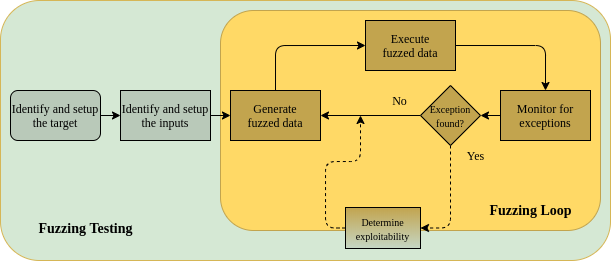
\includegraphics[width=\textwidth]{Chapter2/FuzzingPhases.png}
    \centering
    \caption{Fuzzing phases. Inspired by the definition of Sutton et al. \cite{sutton2007fuzzing}}
    \label{fig:fuzz_phases}
\end{figure}

\textbf{Target} is a software or a combination of executables and hardware \cite{song2019periscope}. A targeted software is any program that a machine can execute. 
Fuzzer needs to know the command for executing the target program and the inputs (arguments) of the program. \textbf{Inputs} are a set of environmental variables, file formats, and any other parameters that affect the execution. The initial seeds of the inputs can guide the fuzzer for finding more complex test cases, yet, it is not mandatory to provide seeds, and a fuzzer can generate valid inputs \textit{out of thin air} \cite{out_of_thin_air}. After the initial setup, the \textbf{fuzzing loop} begins iterating. In each iteration the fuzzer \textbf{executes} the target with the \textbf{provided test cases}. Fuzzer then looks for any exceptions returning from the executions and considers the executed input responsible for causing a \textbf{vulnerability}. The vulnerability can be analyzed for \textbf{exploitability} in the last stage. An exploitable vulnerability can compromise the system and initiate an anomaly.

A common feature in most of the fuzzers is the fuzzing loop which is looking for more valuable inputs. The stages may vary depending on the problem and goals of a fuzzer. We will walk over the stages of AFL as our fuzzer is based on AFL, and we will be back on the stages of fuzzing in the following sections.

\subsubsection*{Sample program}
To evaluate the performance of a fuzzer and assess the execution of it, the sample \textbf{C} code is implemented. (Listing \ref{lst:sample_vul}) \cite{sample_code_ref}

\lstinputlisting[language=C++,style=CodeStyle,caption={Sample vulnerable program},label={lst:sample_vul}]{Codes/Chapter2/sample_vul.c}

The sample program has a \textbf{Heap buffer overflow vulnerability}. If we compile this code with GCC and debugging flags, the vulnerability stays hidden and the program executes without any errors:

\lstinputlisting[language=bash,style=CommandStyle,label={lst:gcc-sample},caption={Compile the sample program}]{Codes/Chapter2/exec_1.txt}

One way to detect the prior vulnerability, is to add AddressSanitizer flag for the compilation \cite{address_san}. ASan is a fast memory error detector. This tool uses memory poisoning for the detection of a heap buffer overflow. (You can find more features of this tool in the reference) \cite{serebryany2012addresssanitizer}

After we provide the ASan flag for the compilation, we face an error with the same input as the previous example (Listing \ref{lst:exec2}):

\lstinputlisting[language=bash,style=CommandStyle,label={lst:exec2}]{Codes/Chapter2/exec_2.txt}

The detection of the vulnerabilities or any other exceptions, signals the operating system for a misbehaviour from the program. A fuzzer would need this signal to evaluate the execution of the target program.

\subsubsection*{Black/Grey/White-box fuzzing}

The \textit{colorful} representation of fuzzers depends on how much information we can collect from any execution of the target. In a blackbox fuzzing, we do not gather any information from the execution, and the fuzzing tries new inputs expecting an error to occur.

\lstinputlisting[language=bash,style=CommandStyle,label={lst:bbox}]{Codes/Chapter2/bbox_fuzz.txt}

% \vspace{1.5\baselineskip}

% Blackbox fuzzer
The introduced fuzzer by Miller \cite{miller1990empirical} was of the very first naive blackbox fuzzers targeting a collection of Unix utilities on different Unix versions. It runs the fuzzing for different lengths of inputs for each utility (of the total 88 utilities) and expects a \textbf{crash}, \textbf{hang}, or a \textbf{succeed} after the execution of the program. The generation of inputs is by the mutation of the inputs' content, and the target program is a blackbox for the fuzzer. As a result, this fuzzer is a mutation-based blackbox fuzzer.


One of the \textbf{downsides} of the blackbox fuzzing is that the program may face some branches with \textbf{magic values}, constraining the variable to a specific set of values; the fuzzer has to apply the exact magic value, which may have a very low probability - it is almost impossible to generate a specific 1 KB string of bytes randomly.. In \cite{banks2006snooze} and \cite{gascon2015pulsar} a set of network protocols are fuzzed in a blackbox manner, but as the target is specified, the performance is enhanced drastically. Any application on the web may be considered a blackboxed program as well, so as \cite{doupe2012enemy} and \cite{duchene2012xss} have targeted web applications and found ways to attack some the websites, looking for different vulnerabilities, such as XSS.

% Whitebox fuzzers
\vspace{1.5\baselineskip}

Whitebox fuzzing works with the source code of the target. In this technique, an \textbf{instrumentation} is applied before the compilation of the program. Instrumeting a program with debugging instructions, is the procedure of injecting new instructions into the resulting binary, without affecting the logic of the program. We will analyze the instrumentations more in the \nameref{sec:2-llvm} section.

The following snippet of code shows an example of such execution \ref{lst:wbox}. \textit{whitebox-instr-c} compiles the program with the required instrumentations and \textit{whitebox-fuzzer} fuzzes the program appropriately.

\lstinputlisting[language=bash,style=CommandStyle,label={lst:wbox}]{Codes/Chapter2/wbox_fuzz.txt}

SAGE, a whitebox fuzzer, was developed as an alternative to blackbox fuzzing to cover the lacks of blackbox fuzzers \cite{godefroid2012sage}. With the benefit of having the source code and internal knowledge for fuzzing, a whitebox fuzzer can leverage symbolic constraints for symbolic analysis to solve the constraints (such as magic values) in the program \cite{cadar2011symbolic}. It can also use dynamic and concolic execution \cite{stephens2016driller} and use taint analysis to locate the regions of seed files influencing values used by program \cite{ganesh2009taint}. In addition, a whitebox fuzzer can find the grammar for parsing the input files without any prior knowledge \cite{godefroid2008grammar}. It is a noticeable performance enhancement as we have the source code.

\vspace{1.5\baselineskip}

Greybox fuzzing resides between whitebox and blackbox fuzzing, as we only have partial knowledge about the internals of the target program. We do not have the source code, but we have some knowledge about the program (for instance, we have the binary file), and as a result, we have the instructions of the program (\ref{lst:gbox}):

\lstinputlisting[language=bash,style=CommandStyle,label={lst:gbox}]{Codes/Chapter2/gbox_fuzz.txt}

AFL \say{allows you to build a standalone feature that leverages the QEMU "user emulation" mode and allows callers to obtain instrumentation output for black-box, closed-source binaries}, working as a greybox fuzzer \cite{afl_qemu}. The instrumentation using \textbf{QEMU} on a binary has an average performance cost of 2-5x, which is better than other tools such as \textbf{DynamoRIO} and \textbf{PIN}.

\subsubsection*{Coverage-based fuzzing}

Coverage-based fuzzing is technique for fuzz testing that instruments the target without analyzing the logic of the program. In a greybox and whitebox coverage-based fuzzing, the instrumentation detects the different paths of the executions \cite{liang2018fuzzing}. AFL instruments the program with only the coverage information (section \nameref{sec:2-afl}).

The instrumentation can collect execution's data such as data coverage, statement coverage, block coverage, decision coverage, and path coverage \cite{yang2009survey}. Bohme et al. \cite{bohme2017coverage} introduced a coverage-based greybox fuzzer that extends AFL and benefits from the Markov Chain model. The fuzzer calculates the \textbf{energy} of the inputs based on the potency of a path for the discovery of new paths.

In another article by Bohme et al. \cite{bohme2017directed}, they introduce their directed fuzzing by the idea of checking the code-coverage for providing inputs that guide the program execution toward some targeted locations. Some of the applications of such a fuzzing approach are patch testing and crash reproduction, which has different use cases compared to a non-directed coverage-based fuzzers.

\subsubsection*{Performance fuzzing}

The \textbf{types} of vulnerabilities that a fuzzer is involved with may be different from other fuzzers. For example, AFL looks for crashes or hangs by selecting and mutating the inputs, and at the same time, it considers the code coverage, size of the inputs, and each execution time of the target program. PerfFuzz \cite{lemieux2018perffuzz} is a greybox fuzzer based on AFL, which aims to generate inputs for executions with higher \textbf{execution time} while using most of the features of AFL in code exploration. PerfFuzz counts how many times each of the edges of the control flow graph (CFG) is executed. Using SlowFuzz \cite{petsios2017slowfuzz}, we can consider any type of resource as a feature to detect the worst-case scenarios (inputs) for a given program. In another project based on AFL, Memlock \cite{wen2020memlock} investigates memory exhaustion by calculating the maximum runtime memory required during executions. A disadvantage in previous works in performance is that the development of the fuzzer for considering different instructions is cumbersome.

\vspace{1.5\baselineskip}

\textbf{Waffle (What An Amazing AFL - WAAAFL)} is a coverage-based whitebox fuzzer that is based on AFL's base code. Waffle leverages \textbf{visitors} to collect the stats of different instructions during the execution. To learn more about Waffle, we study the features we benefit from the LLVM, as well as the current features of AFL that help us in reaching the goals of this thesis.